% ============================================================
%  Memoria TFM — Reconstrucción y reparación 3D de objetos rotos
%  Máster en Big Data, Data Science e Inteligencia Artificial
%
%  INSTRUCCIONES PARA COMPILAR EN OVERLEAF:
%    1. Sube este archivo y referencias.bib al proyecto.
%    2. Crea la carpeta "imagenes/" y sube las imágenes del Word
%       con los nombres indicados en cada \includegraphics.
%    3. Compilador: pdfLaTeX (Settings). Bibliografia: BibTeX (no Biber).
% ============================================================

\documentclass[12pt,a4paper]{report}

% ── Codificación y lengua ────────────────────────────────────────────────────
\usepackage[utf8]{inputenc}
\usepackage[T1]{fontenc}
\usepackage[spanish,es-tabla]{babel}
\usepackage{lmodern}

% ── Márgenes ────────────────────────────────────────────────────────────────
\usepackage[top=2.5cm,bottom=2.5cm,left=2.5cm,right=2.5cm]{geometry}

% ── Tipografía ───────────────────────────────────────────────────────────────
% microtype desactivado: ralentiza mucho la compilación en Overleaf free
% \usepackage{microtype}
\setlength{\parskip}{6pt}
\setlength{\parindent}{0pt}

% ── Matemáticas ──────────────────────────────────────────────────────────────
\usepackage{amsmath,amssymb}

% ── Gráficos e imágenes ──────────────────────────────────────────────────────
\usepackage{graphicx}
\graphicspath{{imagenes/}}        % busca imágenes en la carpeta imagenes/
\usepackage{float}
\usepackage[labelfont=bf,labelsep=period,font=small]{caption}

% ── Tablas ───────────────────────────────────────────────────────────────────
\usepackage{booktabs}
\usepackage{array}
\usepackage{tabularx}
% rotating eliminado — se usa \resizebox en lugar de sidewaystable
\usepackage{threeparttable}   % notas al pie de tabla

% ── Colores ──────────────────────────────────────────────────────────────────
\usepackage[table]{xcolor}
\definecolor{rowgray}{gray}{0.93}

% ── Listas ───────────────────────────────────────────────────────────────────
\usepackage{enumitem}
\usepackage{pifont}
\newcommand{\cmark}{\ding{51}}
\newcommand{\xmark}{\ding{55}}

% ── Encabezados ──────────────────────────────────────────────────────────────
\usepackage{fancyhdr}
\pagestyle{fancy}
\fancyhf{}
\fancyhead[L]{\small\itshape\leftmark}
\fancyhead[R]{\small\thepage}
\renewcommand{\headrulewidth}{0.4pt}

% ── Formato de títulos (chapter = "1. Título") ───────────────────────────────
\usepackage{titlesec}
\titleformat{\chapter}[hang]
  {\Large\bfseries}{\thechapter.}{0.7em}{}
\titlespacing*{\chapter}{0pt}{10pt}{8pt}
\titleformat{\section}[hang]
  {\large\bfseries}{\thesection}{0.7em}{}
\titlespacing*{\section}{0pt}{8pt}{4pt}
\titleformat{\subsection}[hang]
  {\normalsize\bfseries}{\thesubsection}{0.7em}{}
\titlespacing*{\subsection}{0pt}{6pt}{3pt}
\titleformat{\subsubsection}[hang]
  {\normalsize\itshape\bfseries}{\thesubsubsection}{0.7em}{}
\titlespacing*{\subsubsection}{0pt}{5pt}{2pt}

% ── Índice de ecuaciones (con tocloft) ───────────────────────────────────────
\usepackage{tocloft}
\newlistof{myequations}{equ}{Índice de ecuaciones}
\newcommand{\myequations}[1]{%
  \addcontentsline{equ}{myequations}{\protect\numberline{\theequation}#1}%
}
\setlength{\cftmyequationsnumwidth}{2.8em}
\renewcommand{\cftmyequationspresnum}{Ec.\,}
\setlength{\cftmyequationsindent}{0pt}

% ── Hipervínculos ────────────────────────────────────────────────────────────
\usepackage[colorlinks=true,
            linkcolor=blue!50!black,
            citecolor=green!40!black,
            urlcolor=blue!70!black]{hyperref}

% ── Bibliografía: natbib + apalike (no requiere biber, mucho más rápido) ─────
\usepackage[authoryear,round,sort]{natbib}

% ── Código ───────────────────────────────────────────────────────────────────
\usepackage{listings}
\lstset{basicstyle=\ttfamily\small, breaklines=true, frame=single,
        backgroundcolor=\color{gray!8}}

% (imágenes gestionadas con graphicspath — todas en imagenes/)

% ============================================================
\begin{document}

% ── Portada ──────────────────────────────────────────────────────────────────
\begin{titlepage}
  \centering
  \vspace*{1cm}
  
\includegraphics[width=8cm]{logo_master}\\[1.5cm]
  {\large Máster en Big Data, Data Science e Inteligencia Artificial}\\[0.4cm]
  {\large Trabajo Fin de Máster}\\[2.5cm]
  {\LARGE\bfseries Reconstrucción y reparación 3D de objetos rotos}\\[3cm]
  % Foto del objeto (opcional): \includegraphics[width=6cm]{portada_foto}\\[2cm]
  {\large\textbf{Autores}}\\[0.5cm]
  {\large
    Almudena Borreguero Nava\\
    Álvaro Cañete Martí\\
    Luis Corchuelo\\
    Raquel Roca Pereira\\
    Rocío Sánchez Moreno\\
  }

  \vspace{4cm}
  {\large Madrid, septiembre de 2026}
\end{titlepage}

% ── Índices ──────────────────────────────────────────────────────────────────
\tableofcontents
\newpage
\listoffigures
\newpage
\listoftables
\newpage
\listofmyequations
\newpage

% ============================================================
\chapter{Introducción y motivación}
\label{ch:intro}

Muchos objetos de valor, piezas industriales descatalogadas, componentes dañados en
producción o fragmentos arqueológicos llegan a nuestras manos incompletos.
Una pieza de recambio deja de fabricarse y solo queda un ejemplar roto como referencia;
un componente se daña en la cadena de producción y hay que decidir si es reparable o
cuánto material falta.
En estos casos, saber qué forma tenía originalmente el objeto es el primer paso para
actuar sobre él, ya sea para reimprimirlo en~3D, mecanizarlo de nuevo o simplemente
documentarlo.
Tradicionalmente, esta tarea recae en la experiencia de técnicos y especialistas, que
reconstruyen la geometría faltante de forma manual apoyándose en su conocimiento del
objeto y en piezas de referencia similares.
Es un proceso lento, costoso y difícil de escalar.

En paralelo, la visión por computador ha avanzado en la dirección opuesta: en lugar de
restaurar lo que falta, ha aprendido a reconstruir en~3D lo que ya existe.
La reconstrucción tridimensional a partir de imágenes consiste en recuperar la forma de
un objeto en el espacio a partir de una o varias fotografías, y durante décadas se ha
abordado con técnicas geométricas clásicas como la estructura a partir de movimiento
(\textit{structure from motion}) o el estéreo.
En los últimos años, sin embargo, los modelos de aprendizaje profundo han demostrado ser
capaces de predecir una representación 3D completa de un objeto directamente a partir de
imágenes, aprendiendo patrones de forma a partir de grandes colecciones de ejemplos.

Esta capacidad de generalizar a partir de lo aprendido abre una pregunta interesante:
si un modelo de reconstrucción 3D ha aprendido cómo son los objetos completos de una
categoría, ¿podría usar ese conocimiento para inferir la parte que le falta a un objeto
roto, del mismo modo que un técnico experimentado intuye la forma original de una pieza
fragmentada?
Este trabajo explora precisamente esa cuestión: si un modelo entrenado únicamente con
objetos completos puede aprender a restaurarlos digitalmente, generando la geometría
faltante a partir de imágenes de su estado roto.
Una respuesta afirmativa tendría aplicación directa en el control de calidad industrial
y la fabricación de piezas de recambio; y también, de forma más indirecta, en la
documentación del patrimonio, donde un modelo 3D digital permite estudiar una pieza
fragmentada sin intervenir sobre el objeto original.

La arquitectura empleada en este trabajo ha sido Pix2Vox++~\citep{xie2020pix2vox},
una red de reconstrucción 3D basada en redes convolucionales, aplicada sobre imágenes de
categorías de objetos (tazas, botellas, cuencos) tanto en estado completo como roto.

Los objetivos principales del proyecto son:
\begin{itemize}
  \item Evaluar el comportamiento de Pix2Vox++ sobre objetos completos, estudiando el
        efecto del número de vistas de entrada, del \textit{fine-tuning} y de la
        diversidad de categorías de entrenamiento.
  \item Determinar cómo se comporta un modelo entrenado exclusivamente con objetos
        completos al recibir imágenes de un objeto roto.
  \item Crear un modelo de aprendizaje profundo capaz de obtener la representación
        tridimensional completa del objeto reparado, reconstruyendo tanto la parte
        conservada como la faltante.
\end{itemize}

Tras esta introducción, la sección~\ref{ch:conceptos} presenta los conceptos básicos
de reconstrucción 3D.
La sección~\ref{ch:datos} describe los datos y el pipeline de preparación.
Las secciones~\ref{ch:exp_completos} y~\ref{ch:geometrias_rotas} recogen la
experimentación sobre objetos completos y la evaluación sobre geometrías rotas.
La sección~\ref{ch:generativo} presenta el modelo generativo de \textit{shape completion}.
La sección~\ref{ch:malla} describe la generación de malla imprimible.
Finalmente, la sección~\ref{ch:conclusiones} recoge las conclusiones y el trabajo futuro.

% ============================================================
\chapter{Conceptos básicos de reconstrucción 3D}
\label{ch:conceptos}

En esta sección se resumen las nociones necesarias sobre representación 3D: las distintas
formas de codificar un objeto tridimensional, cómo se obtiene esa representación a partir
de imágenes y cómo se evalúa su calidad.

% ── 2.1 ─────────────────────────────────────────────────────────────────────
\section{Formas de representar un objeto en 3D}
\label{sec:representaciones}

Existen varias maneras de representar digitalmente un objeto tridimensional.
Las cuatro empleadas en este trabajo son:

\begin{itemize}
  \item \textbf{Malla (\textit{mesh}):} una superficie formada por vértices, aristas y
        caras triangulares, creando una red que envuelve el objeto.
        Es la representación más común en programas de diseño 3D y la empleada en los
        archivos \texttt{.ply} de este proyecto.

  \item \textbf{Nube de puntos:} conjunto de puntos en el espacio con coordenadas
        $X, Y, Z$, sin conectividad entre ellos.

  \item \textbf{Vóxel:} el equivalente tridimensional de un píxel.
        El espacio se divide en una rejilla regular (en este caso de $32\times32\times32$
        celdas) y cada celda queda ``ocupada'' o ``vacía''.
        Es la representación que predice Pix2Vox++ y la usada como \textit{ground truth}
        durante el entrenamiento.
        El formato \textit{binvox}, utilizado en este trabajo, almacena estas rejillas
        de vóxeles de manera óptima.

  \item \textbf{STL (\textit{Standard Tessellation Language}):} formato de malla
        simplificado orientado a la fabricación aditiva.
        A diferencia de los archivos \texttt{.ply}, el STL solo almacena triángulos:
        cada cara se describe por sus tres vértices y su normal, sin relaciones de
        adyacencia entre triángulos.
        Para que una impresora 3D pueda fabricar el objeto, la malla debe ser
        \textit{watertight} (cerrada y sin huecos).
        Es el formato de salida de la etapa E4 de este proyecto.
\end{itemize}

\begin{figure}[H]
  \centering
  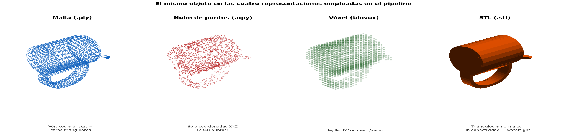
\includegraphics[width=\linewidth]{figura_representaciones}
  \caption{El mismo objeto (taza) en las cuatro representaciones empleadas en el
           pipeline: malla (.ply), nube de puntos (.npy), vóxel (binvox) y STL (.stl).}
  \label{fig:representaciones}
\end{figure}

% ── 2.2 ─────────────────────────────────────────────────────────────────────
\section{Transformación de imágenes 2D en un modelo 3D}
\label{sec:pix2vox}

La arquitectura empleada para predecir la geometría 3D de un objeto a partir de imágenes
es Pix2Vox++~\citep{xie2020pix2vox}.
Este modelo recibe una o varias fotografías del objeto (imágenes RGB de $224\times224$
píxeles) y devuelve, para cada celda de la rejilla de vóxeles, una probabilidad de que
dicha celda esté ocupada.
Al aplicar un umbral se obtiene una rejilla binaria con celdas ocupadas y vacías.

La arquitectura se organiza en cuatro módulos encadenados:
\begin{itemize}
  \item \textbf{Encoder:} red convolucional que extrae características visuales de cada
        imagen de entrada.
        En este trabajo se han empleado ResNet-50~\citep{he2016resnet} preentrenada en
        ImageNet, así como EfficientNet-B4~\citep{tan2019efficientnet}.
  \item \textbf{Decoder:} convierte las características en un volumen preliminar de
        vóxeles para cada vista.
  \item \textbf{Merger:} si hay varias vistas, decide qué partes del volumen predicho
        por cada vista son más fiables y las combina en un único volumen.
  \item \textbf{Refiner:} toma el volumen fusionado y lo corrige, suavizando errores y
        mejorando detalles pequeños.
\end{itemize}

% ── 2.3 ─────────────────────────────────────────────────────────────────────
\section{Evaluación de una reconstrucción óptima}
\label{sec:metricas}

Las métricas empleadas a lo largo del trabajo para evaluar la calidad de las
reconstrucciones 3D son las siguientes.

\subsubsection*{Intersección sobre Unión (IoU)}
Solapamiento entre el volumen de vóxeles predicho ($V_{\text{pred}}$) y el real
($V_{\text{gt}}$).
Varía entre 0 (ninguna coincidencia) y~1 (predicción perfecta).
Es la métrica principal en la fase de reconstrucción con Pix2Vox++.
\begin{equation}
  \mathrm{IoU} = \frac{|V_{\text{pred}} \cap V_{\text{gt}}|}
                      {|V_{\text{pred}} \cup V_{\text{gt}}|}
  \label{eq:iou}
\end{equation}
\myequations{Intersección sobre Unión (IoU)}

\subsubsection*{Distancia de Chamfer (CD-L1)}
Media de las distancias mínimas entre dos nubes de puntos en ambas direcciones.
Un valor menor indica superficies más parecidas.
Es la métrica principal en la fase de \textit{shape completion} (E3).
\begin{equation}
  \mathrm{CD}(P,Q) =
    \frac{1}{|P|}\sum_{p \in P}\min_{q \in Q}\|p-q\|_2 +
    \frac{1}{|Q|}\sum_{q \in Q}\min_{p \in P}\|q-p\|_2
  \label{eq:chamfer}
\end{equation}
\myequations{Distancia de Chamfer (CD-L1)}

\subsubsection*{F-Score a umbral $t$}
Media armónica de la precisión y el recall sobre nubes de puntos para un umbral de
distancia $t$.
Más interpretable que CD y menos sensible a valores atípicos.
Se reporta a $t = 0{,}01\,/\,0{,}02\,/\,0{,}05$ (1--5\,\% de la escala del objeto).
\begin{equation}
  \mathrm{Prec}(t) = \frac{\#\{p\in P : d(p,Q)<t\}}{|P|}
  \label{eq:precision}
\end{equation}
\myequations{Precisión a umbral $t$ (F-Score)}

\begin{equation}
  \mathrm{Rec}(t) = \frac{\#\{q\in Q : d(q,P)<t\}}{|Q|}
  \label{eq:recall}
\end{equation}
\myequations{Recall a umbral $t$ (F-Score)}

\begin{equation}
  F\text{-Score}(t) = \frac{2\cdot\mathrm{Prec}(t)\cdot\mathrm{Rec}(t)}
                          {\mathrm{Prec}(t)+\mathrm{Rec}(t)}
  \label{eq:fscore}
\end{equation}
\myequations{F-Score a umbral $t$}

\subsubsection*{Coeficiente de Sørensen-Dice (DSC)}
Compara el doble de la intersección con la suma de los vóxeles ocupados en el volumen
predicho y en el real.
Varía entre 0 y~1; complementa al IoU siendo más sensible en zonas de alto solapamiento.
\begin{equation}
  \mathrm{DSC} = \frac{2\,|V_{\text{pred}} \cap V_{\text{gt}}|}
                      {|V_{\text{pred}}| + |V_{\text{gt}}|}
  \label{eq:dice}
\end{equation}
\myequations{Coeficiente de Sørensen-Dice (DSC)}

\subsubsection*{Precisión vóxel ($\mathrm{Prec}_{\text{vox}}$)}
Proporción de vóxeles predichos como ocupados que pertenecen realmente al objeto.
Un valor bajo indica que el modelo genera volumen de más (falsos positivos).
\begin{equation}
  \mathrm{Prec}_{\text{vox}} = \frac{|V_{\text{pred}} \cap V_{\text{gt}}|}{|V_{\text{pred}}|}
  \label{eq:prec_vox}
\end{equation}
\myequations{Precisión vóxel}

\subsubsection*{Recall vóxel ($\mathrm{Rec}_{\text{vox}}$)}
Proporción del objeto real que ha sido reconstruida.
Un valor bajo indica que el modelo omite partes de la geometría (falsos negativos).
\begin{equation}
  \mathrm{Rec}_{\text{vox}} = \frac{|V_{\text{pred}} \cap V_{\text{gt}}|}{|V_{\text{gt}}|}
  \label{eq:rec_vox}
\end{equation}
\myequations{Recall vóxel}

% ── 2.4 ─────────────────────────────────────────────────────────────────────
\section{Modelos de aprendizaje profundo empleados en el pipeline}
\label{sec:modelos_pipeline}

El pipeline integra cinco modelos preentrenados, cada uno responsable de una etapa
diferente. Se describen a continuación junto con la etapa donde se usan.

\subsection{SAM --- Segment Anything Model (E1)}
\label{subsec:sam}
Vision Transformer (ViT-H) entrenado sobre más de 1.000\,M de máscaras
\citep{kirillov2023sam}.
Se usa en E1 para eliminar el fondo de las fotografías del objeto roto: a partir de un
punto o caja sobre el objeto, genera la máscara de segmentación que aísla el objeto del
entorno.

\subsection{Pix2Vox++ --- Reconstrucción 3D multi-vista (E2)}
\label{subsec:pix2vox_modelo}
CNN \textit{encoder-decoder} con módulos Merger y Refiner \citep{xie2020pix2vox}.
Toma $N$ imágenes 2D del objeto desde distintos puntos de vista y predice una cuadrícula
de vóxeles $32^3$.
El Merger decide qué partes de cada vista son más fiables y las fusiona; el Refiner
corrige el volumen resultante.
Se parte del modelo preentrenado en ShapeNet con \textit{fine-tuning} sobre vasijas.

\subsection{PCN --- Point Completion Network (E3, baseline)}
\label{subsec:pcn_modelo}
Encoder PointNet~\citep{qi2017pointnet} (MLPs + max-pooling $\rightarrow$ vector global
de 1.024\,d) + decoder FoldingNet~\citep{yang2018foldingnet} en dos etapas: nube gruesa
de 128 puntos $\rightarrow$ expansión a 2.048 mediante \textit{folding} sobre rejilla 2D
\citep{yuan2018pcn}, $\approx$\,4\,M parámetros.
Se entrenó como referencia antes de explorar arquitecturas más complejas.

\subsection{TopNet --- Decoder jerárquico en árbol (E3, exploración)}
\label{subsec:topnet_modelo}
Mismo encoder que PCN, pero con decoder en árbol jerárquico de MLPs: cada nodo se
ramifica en nodos hijo nivel a nivel con \textit{skip connections} al vector global
\citep{tchapmi2019topnet}, $\approx$\,5\,M parámetros.
Su resultado permitió confirmar que el cuello de botella era el vector global y no el
tipo de decoder, motivando el salto a PoinTr.

\subsection{PoinTr --- Point Transformer (E3, modelo principal)}
\label{subsec:pointr_modelo}
Trata la completación como una tarea \textit{sequence-to-sequence} entre grupos de puntos
\citep{yu2021pointr}, 42,2\,M parámetros.
La nube parcial se tokeniza con DGCNN~\citep{wang2019dgcnn}; un
\textit{transformer}~\citep{vaswani2017transformer} encoder-decoder combina esos tokens
con \textit{proxy points} (posiciones estimadas de la región faltante); y una cabeza
\textit{coarse} + FoldingNet local genera la nube completa.
El modelo final (v6\_obj\_sn, 500 épocas, 2.501 pares ShapeNet + Objaverse) obtiene
CD-L1~$= 0{,}0245$ y F-Score~$= 0{,}45$ sobre el conjunto de test.

% ============================================================
\chapter{Datos y pipeline de preparación}
\label{ch:datos}

El entrenamiento de modelos de aprendizaje profundo para la reconstrucción tridimensional
requiere un conjunto de datos rigurosamente estructurado y preprocesado.
En esta sección se describe el origen de los modelos 3D utilizados, los criterios de
filtrado y las transformaciones necesarias para adaptar la información geométrica a los
formatos de entrada y salida de la red neuronal.

% ── 3.1 ─────────────────────────────────────────────────────────────────────
\section{Origen y estructura de los datos}
\label{sec:datos_origen}

Los modelos 3D empleados proceden de ShapeNetCore~\citep{chang2015shapenet}, un
repositorio de más de 51.000 modelos poligonales distribuidos en 55 categorías de
objetos cotidianos.
Este trabajo acota el estudio a la supercategoría de vasijas: objetos con concavidades,
asas y topologías variadas, elegidos porque ShapeNetCore ofrece un volumen suficientemente
amplio de muestras para esta clase.
La hipótesis de partida es que, si el pipeline demuestra una reconstrucción precisa y
generalizable sobre esta familia de objetos, la misma metodología sería extrapolable a
cualquier otra categoría geométrica con volumen de datos equivalente.

De los modelos originales se descartaron mallas degeneradas o demasiado simples (menos
de 1.000 caras) y se simplificaron topológicamente aquellas excesivamente pesadas (más
de 200.000 caras).
Además, cada malla fue trasladada para alinear su centroide con el origen de coordenadas
y escalada proporcionalmente para encajar en un volumen unitario.
El resultado son 2.170 mallas limpias y normalizadas en formato \texttt{.ply},
distribuidas como se muestra en la Tabla~\ref{tab:shapenet}.

\begin{table}[H]
  \centering
  \caption{Distribución de modelos ShapeNet por categoría de vasijas.}
  \label{tab:shapenet}
  \begin{tabular}{lll}
    \toprule
    \textit{Synset} & Categoría & N.º objetos \\
    \midrule
    03593526 & Jarra / tarro     & 545 \\
    03991062 & Maceta             & 489 \\
    02876657 & Botella            & 453 \\
    02747177 & Cubo de basura     & 277 \\
    03797390 & Taza               & 172 \\
    02880940 & Cuenco             & 146 \\
    02946921 & Lata               &  88 \\
    \midrule
    \multicolumn{2}{l}{\textbf{Total}} & \textbf{2.170} \\
    \bottomrule
  \end{tabular}
\end{table}

Este conjunto se emplea en las fases~1 y~2 del proyecto (capítulos~\ref{ch:exp_completos}
y~\ref{ch:geometrias_rotas}) para entrenar y evaluar Pix2Vox++ sobre objetos completos
y sobre geometrías rotas.

Además de estas 2.170 mallas, el proyecto emplea otros dos repositorios en la fase de
\textit{shape completion} (capítulo~\ref{ch:generativo}), donde el problema deja de ser
reconstruir un objeto desde imágenes y pasa a ser completar una nube de puntos parcial.

\subsubsection*{Objaverse \textnormal{\citep{deitke2023objaverse}}}
Es un repositorio de código abierto con más de 800.000 modelos 3D anotados, de calidad
y estilo muy heterogéneos.
A diferencia de ShapeNet, no está organizado en categorías rígidas: los objetos provienen
de artistas y estudios de diseño, lo que aporta mayor variedad geométrica y visual.
De este repositorio se seleccionaron y limpiaron 131 mallas de la supercategoría de
vasijas (tazas, jarras, cuencos), aplicando los mismos criterios de filtrado que para
ShapeNet.
Estos modelos se emplean exclusivamente como objetos completos para generar roturas
sintéticas adicionales en E3; no existen pares de rotura reales en Objaverse.

\subsubsection*{Fantastic Breaks \textnormal{\citep{lamb2023fantastic}}}
Es el único de los tres \textit{datasets} que ofrece pares reales (fragmento roto,
objeto completo) en lugar de roturas sintéticas.
Contiene 150 objetos domésticos físicamente rotos, escaneados en 3D junto con sus
contrapartes completas mediante un escáner de luz estructurada.
Las nubes de puntos resultantes presentan ruido de escáner, densidad irregular y pequeñas
inconsistencias de alineación entre el fragmento y el objeto completo.
De este conjunto se filtraron los pares de la supercategoría de vasijas (\textit{mug,
bowl, jar, cup}), obteniendo 61 pares utilizables.
La alineación previa de cada par se realizó aplicando la transformación incluida en los
metadatos del \textit{dataset} y refinándola con ICP
(\textit{Iterative Closest Point}), ya que fragmento y objeto completo provienen de
escaneos independientes.
Dado su tamaño reducido (61 pares frente a los 2.501 sintéticos del conjunto final),
se usa principalmente como conjunto de evaluación en condiciones reales y, de forma
experimental, como datos de entrenamiento adicional.

% ── 3.2 ─────────────────────────────────────────────────────────────────────
\section{Conversión de la malla al \textit{ground truth}: de PLY a binvox}
\label{sec:ply_binvox}

Dado que Pix2Vox++ predice una rejilla volumétrica binaria y no una malla, cada modelo
\texttt{.ply} se convirtió en un volumen \texttt{model.binvox} de resolución
$32\times32\times32$ mediante la herramienta binvox~\citep{min2004binvox}.
El proceso solidifica el interior del objeto deteniendo el llenado un vóxel antes de
alcanzar la superficie de la malla, evitando así huecos internos, y se complementa con
un renderizado adicional en modo contorno que preserva partes finas y estrechas ---como
las asas--- que de otro modo desaparecerían al reducir la resolución a $32^3$
(Figura~\ref{fig:binvox}).
El objeto se centra siempre en la misma posición del cubo de vóxeles, garantizando la
correspondencia espacial con las imágenes de entrada.
Los datos resultantes, comprimidos mediante \textit{run-length encoding}, se descomprimen
y se transponen del orden interno de binvox ($X,Z,Y$) al orden ($X,Y,Z$) que espera
Pix2Vox++.

\begin{figure}[H]
  \centering
  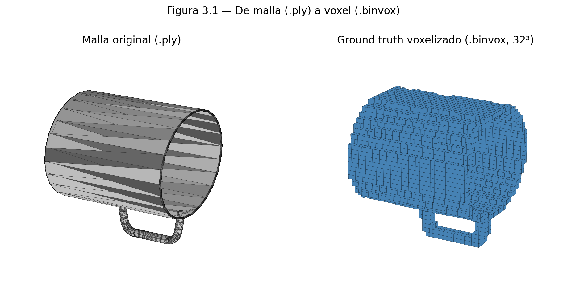
\includegraphics[width=0.85\linewidth]{imagen_binvox}
  \caption{Proceso de voxelización: malla \texttt{.ply} original (izquierda) y
           volumen binvox $32^3$ resultante (derecha).}
  \label{fig:binvox}
\end{figure}

% ── 3.3 ─────────────────────────────────────────────────────────────────────
\section{Generación de datos de entrada: renderizado de vistas 2D}
\label{sec:renderizado}

Dado que Pix2Vox++ requiere imágenes bidimensionales como datos de entrada, se generan
vistas 2D sintéticas mediante BlenderProc~\citep{denninger2020blenderproc}, garantizando
la correspondencia espacial exacta con el \textit{ground truth}
(Figura~\ref{fig:blenderproc}).
Para que el modelo se centre en la inferencia de la geometría y no sufra sesgos por las
texturas originales de ShapeNet, se aplica un material neutro homogéneo a todos los
objetos, con iluminación fija de tres puntos.
Para cada objeto se capturan 20 vistas reproducibles (8 a 20° de elevación, 8 a 40°
y 4 a 60°, radio 2,2), en formato RGBA a $224\times224$\,px, normalizadas después
a $[-1, 1]$.
Este repertorio permite evaluar el modelo con distintos números de vistas de entrada
(1, 5 o 20 vistas), tomando siempre subconjuntos fijos y reproducibles.

\begin{figure}[H]
  \centering
  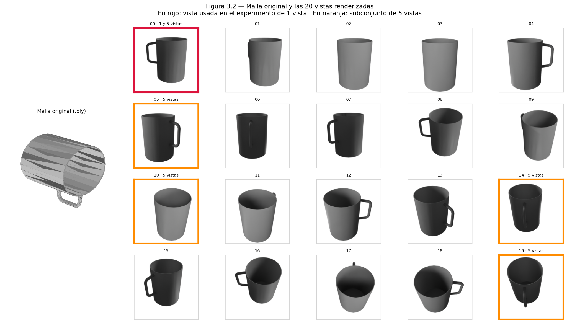
\includegraphics[width=0.85\linewidth]{imagen_blenderproc}
  \caption{Vistas 2D sintéticas generadas con BlenderProc para un mismo objeto desde
           20 ángulos distintos. Las imágenes son RGBA $224\times224$\,px.}
  \label{fig:blenderproc}
\end{figure}

% ── 3.4 ─────────────────────────────────────────────────────────────────────
\section{División del conjunto de datos}
\label{sec:split}

Los 2.170 objetos validados se dividieron en tres subconjuntos independientes:
entrenamiento (70\,\%), validación (15\,\%) y test (15\,\%).
La partición se realizó a nivel de objeto, no de imagen: las 20 vistas de un mismo
modelo pertenecen de forma indivisible a un único subconjunto, evitando así
\textit{data leakage}.

% ============================================================
\chapter{Experimentación sobre objetos completos}
\label{ch:exp_completos}

Esta fase evalúa la capacidad del modelo para reconstruir objetos tridimensionales
completos a partir de imágenes RGB renderizadas.
El objetivo es determinar cómo influyen tres factores clave en la calidad de la
reconstrucción:
\begin{itemize}
  \item Número de vistas disponibles por objeto (1, 5 o 20 imágenes).
  \item Aplicación o no de \textit{fine-tuning} sobre la categoría objetivo.
  \item Ampliación del conjunto de categorías utilizadas en el entrenamiento.
\end{itemize}

Todos los experimentos se realizan sobre objetos completos con sus 20 vistas y su
\textit{ground truth} voxelizado.
Las divisiones de entrenamiento, validación y test se mantienen constantes, evitando
fugas de información entre subconjuntos.

% ── 4.1 ─────────────────────────────────────────────────────────────────────
\section{Número de vistas y necesidad de \textit{fine-tuning}}
\label{sec:vistas_finetuning}

\subsection{Descripción general}
\label{subsec:descripcion_exp}

Los primeros experimentos evalúan el comportamiento del modelo preentrenado sin ajuste
adicional, utilizando únicamente la categoría de tazas.
Se prueban tres configuraciones: 1 vista, 5 vistas y 20 vistas por objeto.
Para garantizar la comparabilidad, se emplean las mismas vistas de referencia en todas
las evaluaciones.

Posteriormente, se repite la misma comparación aplicando \textit{fine-tuning},
ajustando los pesos del modelo sobre el conjunto de entrenamiento de tazas.
El \textit{fine-tuning} incorpora:
\begin{itemize}
  \item Tasas de aprendizaje diferenciadas para \textit{encoder} y \textit{decoders}.
  \item \textit{Batch Normalization} activada en el \textit{encoder}.
  \item Recorte de gradiente (\textit{gradient clipping}) para estabilizar el
        entrenamiento.
  \item \textit{Scheduler} con reducción de la tasa de aprendizaje cuando la métrica
        IoU no mejora.
  \item \textit{Early stopping} basado en validación para evitar sobreajuste.
\end{itemize}

Todos los entrenamientos se ejecutan sobre la GPU A100 de Google Colab.

\subsection{Resultados: sin \textit{fine-tuning} vs.\ con \textit{fine-tuning}}
\label{subsec:resultados_finetuning}

\begin{figure}[H]
  \centering
  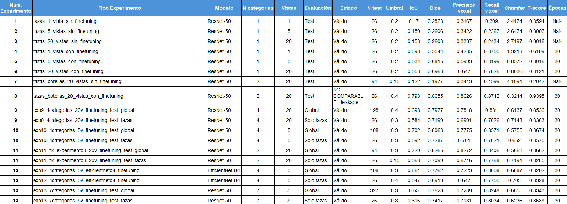
\includegraphics[width=0.85\linewidth]{imagen_tabla_finetuning}
  \caption{Tabla comparativa de IoU para los tres números de vistas (1, 5, 20) con y
           sin \textit{fine-tuning} sobre la categoría de tazas.}
  \label{fig:tabla_finetuning}
\end{figure}

\subsection{Interpretación de resultados}
\label{subsec:interpretacion_finetuning}

\subsubsection*{Sin \textit{fine-tuning}}
\begin{itemize}
  \item Con 1 vista, el modelo preentrenado ofrece reconstrucciones muy limitadas.
  \item Con 5 vistas, la reconstrucción mejora, pero sigue siendo insuficiente para
        capturar detalles finos.
  \item Con 20 vistas, el modelo logra reconstrucciones razonables, aunque todavía
        presenta huecos y errores en la geometría.
\end{itemize}

\subsubsection*{Con \textit{fine-tuning}}
\begin{itemize}
  \item El salto de calidad es notable incluso con 1 vista.
  \item Con 5 vistas, el modelo alcanza un equilibrio excelente entre coste
        computacional y calidad de reconstrucción.
  \item Con 20 vistas, se obtienen las mejores métricas dentro de esta primera fase.
\end{itemize}

En conjunto, el \textit{fine-tuning} demuestra ser indispensable para adaptar
Pix2Vox++ a la categoría de tazas, especialmente cuando el número de vistas es reducido.

% ── 4.2 ─────────────────────────────────────────────────────────────────────
\section{Empleo de más categorías en entrenamiento}
\label{sec:mas_categorias}

Tras evaluar el comportamiento del modelo exclusivamente sobre tazas, se amplía el
conjunto de entrenamiento incorporando nuevas categorías de ShapeNet:
\begin{itemize}
  \item Dos categorías: tazas + botellas (experimentos~7 y~11).
  \item Cuatro categorías (experimentos~9 y~10).
  \item Siete categorías (experimento~13).
  \item Seis categorías (experimento~14, variante del~13 sin macetas).
\end{itemize}

Se realizan dos evaluaciones: específica sobre tazas, y global sobre todas las categorías
usadas en el entrenamiento.

\subsection{Resultados con más categorías}
\label{subsec:resultados_categorias}

\begin{figure}[H]
  \centering
  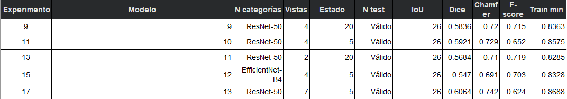
\includegraphics[width=0.85\linewidth]{imagen_tabla_categorias}
  \caption{Tabla comparativa de IoU para los experimentos con múltiples categorías de
           entrenamiento.}
  \label{fig:tabla_categorias}
\end{figure}

\subsection{Interpretación de resultados}
\label{subsec:interpretacion_categorias}

Los resultados muestran que con siete categorías, el modelo alcanza su mejor rendimiento
global, especialmente en el experimento~13 (cinco vistas, \textit{fine-tuning} y siete
categorías), donde se observa mayor robustez ante variaciones geométricas, mejor
consistencia en la reconstrucción de tazas e IoU más alta tanto en evaluación específica
como global.
El experimento~14 (seis categorías) confirma la tendencia: eliminar una categoría no
mejora los resultados.

% ── 4.3 ─────────────────────────────────────────────────────────────────────
\section{Sustitución de la red neuronal del \textit{encoder}}
\label{sec:encoder_eficientnet}

En el experimento~12 se evalúa la sustitución del \textit{encoder} original de
Pix2Vox++ por EfficientNet-B4~\citep{tan2019efficientnet}.
Este experimento se descarta por varios motivos: el \textit{encoder} requiere un
preprocesamiento distinto al de Pix2Vox++, rompiendo la compatibilidad con el pipeline
original; la memoria GPU necesaria excede los recursos disponibles en Colab; y las
primeras pruebas muestran inestabilidad en el entrenamiento sin mejoras significativas
en IoU.

% ── 4.4 ─────────────────────────────────────────────────────────────────────
\section{Resumen de esta fase}
\label{sec:resumen_exp}

La configuración óptima seleccionada es el \textbf{Experimento~13}: cinco vistas,
\textit{fine-tuning} y siete categorías.
Destaca por el equilibrio óptimo entre coste computacional y calidad de reconstrucción,
mejor IoU global y específica sobre tazas, mayor robustez ante variaciones geométricas, y
reconstrucciones visualmente más completas con menos huecos y mejor definición de bordes.

\begin{figure}[H]
  \centering
  \begin{tabular}{ccc}
    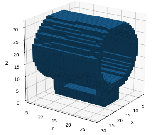
\includegraphics[width=0.28\linewidth]{imagen_taza_real} &
    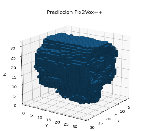
\includegraphics[width=0.28\linewidth]{imagen_pred_exp4} &
    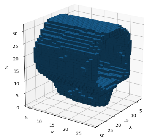
\includegraphics[width=0.28\linewidth]{imagen_pred_exp13} \\
    \small Taza real &
    \small Predicción exp.~4 &
    \small Predicción exp.~13 \\
  \end{tabular}
  \caption{Comparativa visual entre la taza real y las predicciones de los
           experimentos~4 y~13.}
  \label{fig:comp_exps}
\end{figure}

% ============================================================
\chapter{Evaluación sobre geometrías rotas}
\label{ch:geometrias_rotas}

Una vez seleccionado el mejor modelo de Pix2Vox++ sobre objetos completos, se evaluó
su capacidad para generalizar a un escenario radicalmente distinto: geometrías
parcialmente destruidas.
El objetivo era comprobar si una red entrenada exclusivamente para reconstruir volúmenes
completos podía inferir correctamente la forma de una pieza rota a partir únicamente de
sus imágenes 2D, y en qué medida un reentrenamiento dirigido podía cerrar esa brecha.

% ── 5.1 ─────────────────────────────────────────────────────────────────────
\section{Metodología con datos reales: BPA y Fantastic Breaks}
\label{sec:bpa_fb}

El enfoque inicial se basó en el conjunto de datos Fantastic Breaks~\citep{lamb2023fantastic},
que contiene nubes de puntos 3D obtenidas de escaneos de tazas reales con fracturas físicas.
Dado que Pix2Vox++ requiere imágenes 2D como entrada, era necesario convertir estas nubes
discontinuas en mallas sólidas \texttt{.ply} renderizables mediante BlenderProc.
Para ello se empleó el algoritmo Ball Pivoting~\citep{bernardini1999ball} (BPA).

Su aplicación sobre datos reales rotos presentó dos problemas insalvables:
BPA no conseguía cerrar las transiciones abruptas de la fractura, generando artefactos
severos; y obtener una malla renderizable sin agujeros exigía aplicar algoritmos de
cierre volumétrico que ``curaban'' la zona de la rotura, devolviendo al objeto su forma
completa y destruyendo el propósito de la prueba.

% ── 5.2 ─────────────────────────────────────────────────────────────────────
\section{Metodología con roturas sintéticas y \textit{fine-tuning}}
\label{sec:roturas_sinteticas}

Ante la imposibilidad de usar las nubes reales sin distorsionar la geometría, se optó
por generar roturas sintéticas sobre las mallas \texttt{.ply} intactas ya empleadas para
entrenar Pix2Vox++ (172 tazas).
Cada objeto se interseca con un plano 3D de orientación y posición aleatorias, validando
que la pieza resultante conserve entre el 25\,\% y el 85\,\% de los vértices originales
para garantizar que siga siendo reconocible.
A diferencia de BPA, este método produce bordes de fractura completamente limpios y
\textit{watertight}, listos para generar de forma fiable las cinco vistas de entrada
(Figura~\ref{fig:rotura_sintetica}).

\begin{figure}[H]
  \centering
  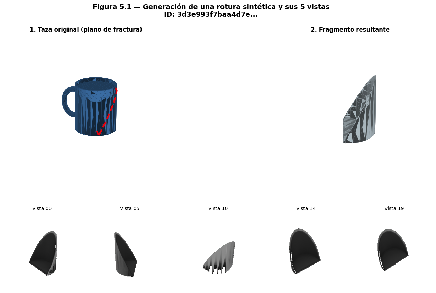
\includegraphics[width=0.75\linewidth]{imagen_rotura_sintetica}
  \caption{Ejemplo de taza con rotura sintética y las cinco vistas de entrada
           generadas con BlenderProc.}
  \label{fig:rotura_sintetica}
\end{figure}

% ── 5.3 ─────────────────────────────────────────────────────────────────────
\section{Resultado: evaluación \textit{zero-shot} y \textit{fine-tuning}}
\label{sec:resultados_roturas}

Sobre este nuevo conjunto se evaluó primero el modelo base (experimento~13), entrenado
exclusivamente con tazas completas, sin ningún ajuste adicional (evaluación
\textit{zero-shot}).
El resultado confirmó una capacidad de generalización prácticamente nula: IoU medio
de~0,054 y Dice de~0,098 sobre las 172 tazas rotas.

Se realizó entonces \textit{fine-tuning}: se generaron 532 variantes de rotura
adicionales para entrenamiento y validación, reservando las 26 tazas de test ya
evaluadas para comparar directamente el antes y el después.
La evaluación final (Tabla~\ref{tab:roturas}) confirma el efecto de la adaptación.

\begin{table}[H]
  \centering
  \caption{Rendimiento comparativo en la reconstrucción de tazas rotas (test set,
           26 tazas).}
  \label{tab:roturas}
  \begin{tabular}{lccc}
    \toprule
    Modelo evaluado & IoU medio & Coef.\ Dice & Mejora (IoU) \\
    \midrule
    Base (solo tazas completas)     & 0,0553 & 0,1009 & --- \\
    \textit{Fine-tuneado} (roturas) & 0,3113 & 0,4544 & +0,2560 \\
    \bottomrule
  \end{tabular}
\end{table}

El modelo \textit{fine-tuneado} multiplica por casi seis el IoU del modelo base, y mejora
en 25 de las 26 tazas evaluadas.
Pese a la mejora sustancial, el modelo dista de una reconstrucción perfecta (Dice~$= 0{,}45$):
las limitaciones se discuten en la Sección~\ref{sec:limitaciones}.

\begin{figure}[H]
  \centering
  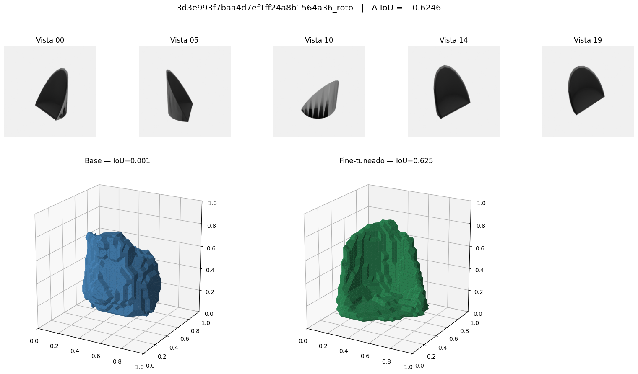
\includegraphics[width=0.85\linewidth]{imagen_comparativa_finetuning}
  \caption{Comparativa visual entre las predicciones del modelo base y el modelo
           \textit{fine-tuneado} sobre tres tazas rotas del test set.}
  \label{fig:comp_finetuning}
\end{figure}

% ============================================================
\chapter{Creación del modelo generativo para la reconstrucción del objeto roto}
\label{ch:generativo}

\section{Motivación y enfoque del problema}
\label{sec:motivacion_generativo}

El capítulo anterior mostró que Pix2Vox++ generaliza bien a objetos rotos, pero
reconstruye la forma \textit{actual} del fragmento, con la región dañada ausente.
El pipeline necesita, en cambio, la geometría \textit{original} del objeto, previa a la
rotura, para poder imprimir la pieza de repuesto.

Esta diferencia ---reconstruir lo que hay frente a completar lo que falta--- define la
tarea de \textit{shape completion}.
El problema se formula así: dada una nube de puntos parcial que representa un fragmento
de un objeto, predecir la nube de puntos completa del objeto original antes del daño.
Las etapas E1 y E2 obtienen la nube parcial a partir de las fotos; E3 la completa.

\begin{center}
Fotos del objeto roto $\to$ \textbf{E1} (SAM + COLMAP) $\to$
\textbf{E2} (Pix2Vox++) $\to$ nube parcial (2.048 pts) $\to$
\textbf{E3} (PoinTr) $\to$ nube completa $\to$
\textbf{E4} $\to$ STL imprimible
\end{center}

El enfoque es supervisado: se entrena con pares (nube rota, nube completa), generando
las nubes rotas sintéticamente para simular la salida esperada de E2.
Se compararon tres arquitecturas de complejidad creciente (PCN, TopNet, PoinTr) con el
mismo \textit{dataset} y protocolo.

\subsection{Interfaz con E2: conversión de vóxeles a nube de puntos}
\label{subsec:interfaz_e2_e3}

Pix2Vox++ produce como salida una cuadrícula de vóxeles $32^3$.
Este formato no es directamente compatible con la entrada de E3, que espera una nube XYZ
de forma $(2048,3)$, centrada en el origen y escalada a esfera unidad.
El paso de conversión tiene cuatro etapas:
\begin{enumerate}
  \item \textbf{Umbralización:} se aplica un umbral de~0,5 sobre la cuadrícula para
        obtener una máscara binaria de ocupación.
  \item \textbf{Extracción de coordenadas:} las celdas ocupadas se convierten en
        puntos 3D.
  \item \textbf{Normalización:} el conjunto se centra en el centroide y se escala a
        esfera unidad.
  \item \textbf{Submuestreo a 2.048 puntos:} si hay más celdas ocupadas, se aplica
        \textit{furthest point sampling} (FPS).
\end{enumerate}

Esta conversión tiene una limitación: la resolución $32^3$ implica que los puntos del
resultado solo pueden ocupar posiciones múltiplos de $1/32\approx 0{,}031$ unidades.
En objetos con geometría fina (asas, bordes delgados), esto puede perder detalle
geométrico capturado implícitamente por E2.
Esta diferencia de dominio es una fuente de error adicional en producción.

% ── 6.2 ─────────────────────────────────────────────────────────────────────
\section{Datos de entrenamiento para \textit{shape completion}}
\label{sec:datos_e3}

\subsection{Datasets}
\label{subsec:datasets_e3}

Los \textit{datasets} empleados ---ShapeNet, Objaverse y Fantastic Breaks--- se describen
en la Sección~\ref{sec:datos_origen}.
Tras el proceso de generación y limpieza de roturas, el \textit{dataset} final para E3
contiene 60 pares de Fantastic Breaks, 855 de ShapeNet y 397 de Objaverse.

\subsection{Generación de roturas sintéticas}
\label{subsec:roturas_sinteticas_e3}

Partiendo de una nube densa (20.000 puntos) sobre cada malla limpia, se simula la pérdida
de una porción del objeto mediante un corte con plano de orientación y posición aleatorias:
se proyectan los puntos sobre la normal del plano y se descarta el lado que supere un
percentil de corte, ajustado para eliminar entre el 10\,\% y el 40\,\% de la superficie.
También se probaron variantes de corte esférico e intersección de dos planos, para
diversificar los patrones de rotura.
Cada rotura se valida antes de aceptarse, descartando casos con nube colapsada, degenerada
en un plano o dividida en grupos desconectados.

\begin{figure}[H]
  \centering
  \begin{tabular}{cc}
    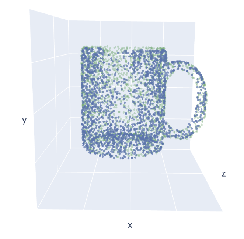
\includegraphics[width=0.42\linewidth]{imagen_rotura_real} &
    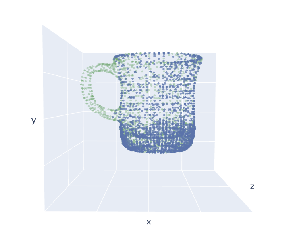
\includegraphics[width=0.42\linewidth]{imagen_rotura_sintetica_sn} \\
    \small Rotura real (Fantastic Breaks) &
    \small Rotura sintética (ShapeNet) \\
  \end{tabular}
  \caption{Comparativa entre una rotura real de Fantastic Breaks (nube de escáner) y
           una rotura sintética generada por corte de plano sobre ShapeNet.}
  \label{fig:roturas_comp}
\end{figure}

\subsection{Preprocesamiento y \textit{data loader}}
\label{subsec:preprocesamiento}

Todos los pares se llevan a un formato común: nubes de 2.048 puntos XYZ (float32),
centradas en el origen y escaladas al percentil~99 de la distancia al centro
(en vez de la distancia máxima absoluta, para evitar que un punto atípico distorsione
la escala).
Se guardan como ficheros \texttt{.npy}, de modo que el \textit{data loader} trata igual
pares reales y sintéticos.
Fantastic Breaks requirió alineación previa con ICP entre fragmento y modelo completo,
tal como se detalla en la Sección~\ref{sec:datos_origen}.

% ── 6.4 ─────────────────────────────────────────────────────────────────────
\section{Baseline: PCN}
\label{sec:pcn}

\subsection{Arquitectura}
\label{subsec:pcn_arq}

La arquitectura de PCN se describe en la Sección~\ref{subsec:pcn_modelo}.
En este proyecto se configura para generar 2.048 puntos (en vez de los 16.384 originales),
con una nube gruesa intermedia de 128 puntos.
Se usó la implementación \texttt{qinglew/PCN-PyTorch}.

\subsection{Experimentos y resultados}
\label{subsec:pcn_exp}

El baseline se entrenó de forma incremental (v1 a v5), corrigiendo en cada iteración un
problema detectado en la anterior.

\begin{table}[H]
  \centering
  \caption{Experimentos del baseline PCN.
           Mejor resultado en \textbf{negrita}.}
  \label{tab:pcn}
  \begin{tabular}{llp{5cm}cc}
    \toprule
    Versión & Datos & Cambios & CD-L1 $\downarrow$ & F-Score $\uparrow$ \\
    \midrule
    v1 & FB + sint.\ & Primer entrenamiento, 100 épocas      & 0,0766 & 0,019 \\
    v3 & FB + sint.\ & 400 épocas                            & 0,0665 & 0,024 \\
    v4 & FB + sint.\ & Filtro \textit{outliers}, más peso
                      rama \textit{coarse}                   & 0,0641 & 0,024 \\
    v5 & FB + sint.\ & Corrección desalineación de centroide & \textbf{0,0630} & \textbf{0,026} \\
    \bottomrule
  \end{tabular}
  \begin{tablenotes}\footnotesize
    \item La v2 no aparece: fue un intento con bug en la pérdida, detectado y descartado
          antes de completarse.
  \end{tablenotes}
\end{table}

El cambio más relevante fue el de v4 a v5: al activar \texttt{CENTRAR\_EN\_ROTO=True},
cada par se recentra por el centroide del fragmento antes de pasarlo a la red.
Sin esta corrección, el desplazamiento de $\approx0{,}4$ unidades entre el centroide del
fragmento y el origen del objeto completo hace que el modelo colapse a una placa plana
(CD~$\approx 0{,}18$--$0{,}23$).
Este principio se mantuvo en todos los experimentos posteriores.

Aun así, v5 alcanza F-Score~$= 0{,}026$, lejos de resultados aceptables.
Una prueba de sobreajuste a un único ejemplo real confirmó que la limitación es más del
decoder tipo \textit{folding} que de los datos, motivando la exploración de TopNet y
finalmente PoinTr.

\begin{figure}[H]
  \centering
  \begin{tabular}{cccc}
    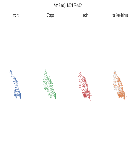
\includegraphics[width=0.22\linewidth]{pcn_muestra1} &
    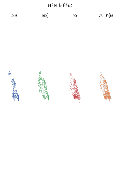
\includegraphics[width=0.22\linewidth]{pcn_muestra2} &
    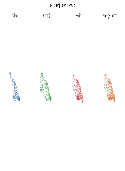
\includegraphics[width=0.22\linewidth]{pcn_muestra3} &
    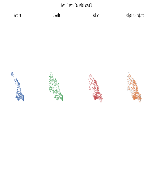
\includegraphics[width=0.22\linewidth]{pcn_muestra4} \\
  \end{tabular}
  \caption{Mejor caso del test de PCN (CD$=0{,}029$, F-Score$=0{,}049$):
           fragmento de entrada, predicción y \textit{ground truth}.}
  \label{fig:pcn_mejor}
\end{figure}

% ── 6.5 ─────────────────────────────────────────────────────────────────────
\section{Exploración con TopNet}
\label{sec:topnet}

\subsection{Arquitectura}
\label{subsec:topnet_arq}

La arquitectura de TopNet se describe en la Sección~\ref{subsec:topnet_modelo}.
Se implementó en PyTorch puro, sin extensiones CUDA, para aislar si el techo bajo
de PCN se debía al \textit{decoder} o al \textit{encoder}: al compartir el mismo
\textit{encoder} que PCN, cualquier diferencia de resultado es atribuible únicamente
al \textit{decoder}.

\subsection{Experimentos y resultados}
\label{subsec:topnet_exp}

TopNet se entrenó con la misma mezcla de datos y el mismo \textit{fix} de centroide
que PCN~v5, para que la comparación fuera controlada.

\begin{table}[H]
  \centering
  \caption{Comparativa PCN vs.\ TopNet con la misma configuración de datos.}
  \label{tab:topnet}
  \begin{tabular}{lcc}
    \toprule
    Modelo & CD-L1 $\downarrow$ & F-Score $\uparrow$ \\
    \midrule
    PCN v5  & 0,0630 & 0,0257 \\
    TopNet  & 0,060  & 0,0329 \\
    \bottomrule
  \end{tabular}
\end{table}

Este resultado confirma que el \textit{decoder} tipo \textit{folding} de PCN era,
al menos parcialmente, un factor limitante.
Con todo, la mejora sigue siendo moderada (F-Score $= 0{,}033$), y no cierra la
brecha necesaria.
Esto motivó el salto a PoinTr, que sustituye tanto el \textit{encoder} como el
\textit{decoder} por un mecanismo de atención entre puntos.

% ── 6.6 ─────────────────────────────────────────────────────────────────────
\section{Modelo principal: PoinTr}
\label{sec:pointr}

\subsection{Arquitectura}
\label{subsec:pointr_arq}

La arquitectura de PoinTr se describe en la Sección~\ref{subsec:pointr_modelo}.
Se usó la implementación oficial (\texttt{yuxumin/PoinTr}).
Las extensiones CUDA (\texttt{chamfer\_dist}, \texttt{pointnet2\_ops}, \texttt{knn\_cuda})
se sustituyeron por versiones en PyTorch puro para compatibilidad con Google Colab
(coste: $\times1{,}4$ en velocidad).

\subsection{Experimentos y evolución de resultados}
\label{subsec:pointr_exp}

PoinTr se entrenó en seis versiones principales, cada una corrigiendo o extendiendo la
anterior.
La tabla completa de todos los experimentos del proyecto figura en la
Tabla~\ref{tab:experimentos_e3} del Anexo~\ref{ap:tablas}.

\paragraph{Los datos, no la arquitectura, son el factor dominante.}
La evolución de PoinTr~v4 (CD$=0{,}0569$, 61 pares reales) $\to$
v5\_obj (CD$=0{,}0306$, 397 pares Objaverse) $\to$
v6\_obj\_sn (CD$=0{,}0245$, 2.501 pares con ShapeNet) replica lo observado en PCN:
más datos limpios y bien alineados mejoran el modelo más que cualquier cambio de
arquitectura o hiperparámetros a este volumen.

\paragraph{Fantastic Breaks perjudica a esta escala.}
Al añadir sus 60 pares reales al mejor modelo (v6\_fb\_obj\_sn), el CD empeora de
0,0245 a~0,0297 (+21\,\%).
La diferencia de distribución entre datos reales (ruido de escáner, densidad irregular)
y los 2.501 pares sintéticos (densidad y orientación uniformes) hace que, a este volumen,
60 pares reales actúen como ruido.
Esto es relevante para la integración final: al recibir E3 nubes reales de E2, el
rendimiento puede ser peor que en el test set sintético.

\paragraph{Alineación de centroide (hallazgo crítico).}
Al generar roturas sintéticas, el centroide del fragmento se desplaza hasta
$\approx0{,}4$ unidades del origen del objeto completo.
Sin corregirlo, el modelo debía aprender esa traslación implícitamente, colapsando en
los peores casos a una placa plana (CD~$\approx 0{,}18$--$0{,}23$).
La solución ---centrar el fragmento en su propio centroide y desplazar el
\textit{ground truth} al mismo sistema de referencia--- se implementó desde PCN~v5 y
se mantuvo en todos los experimentos de PoinTr desde v4.

\begin{figure}[H]
  \centering
  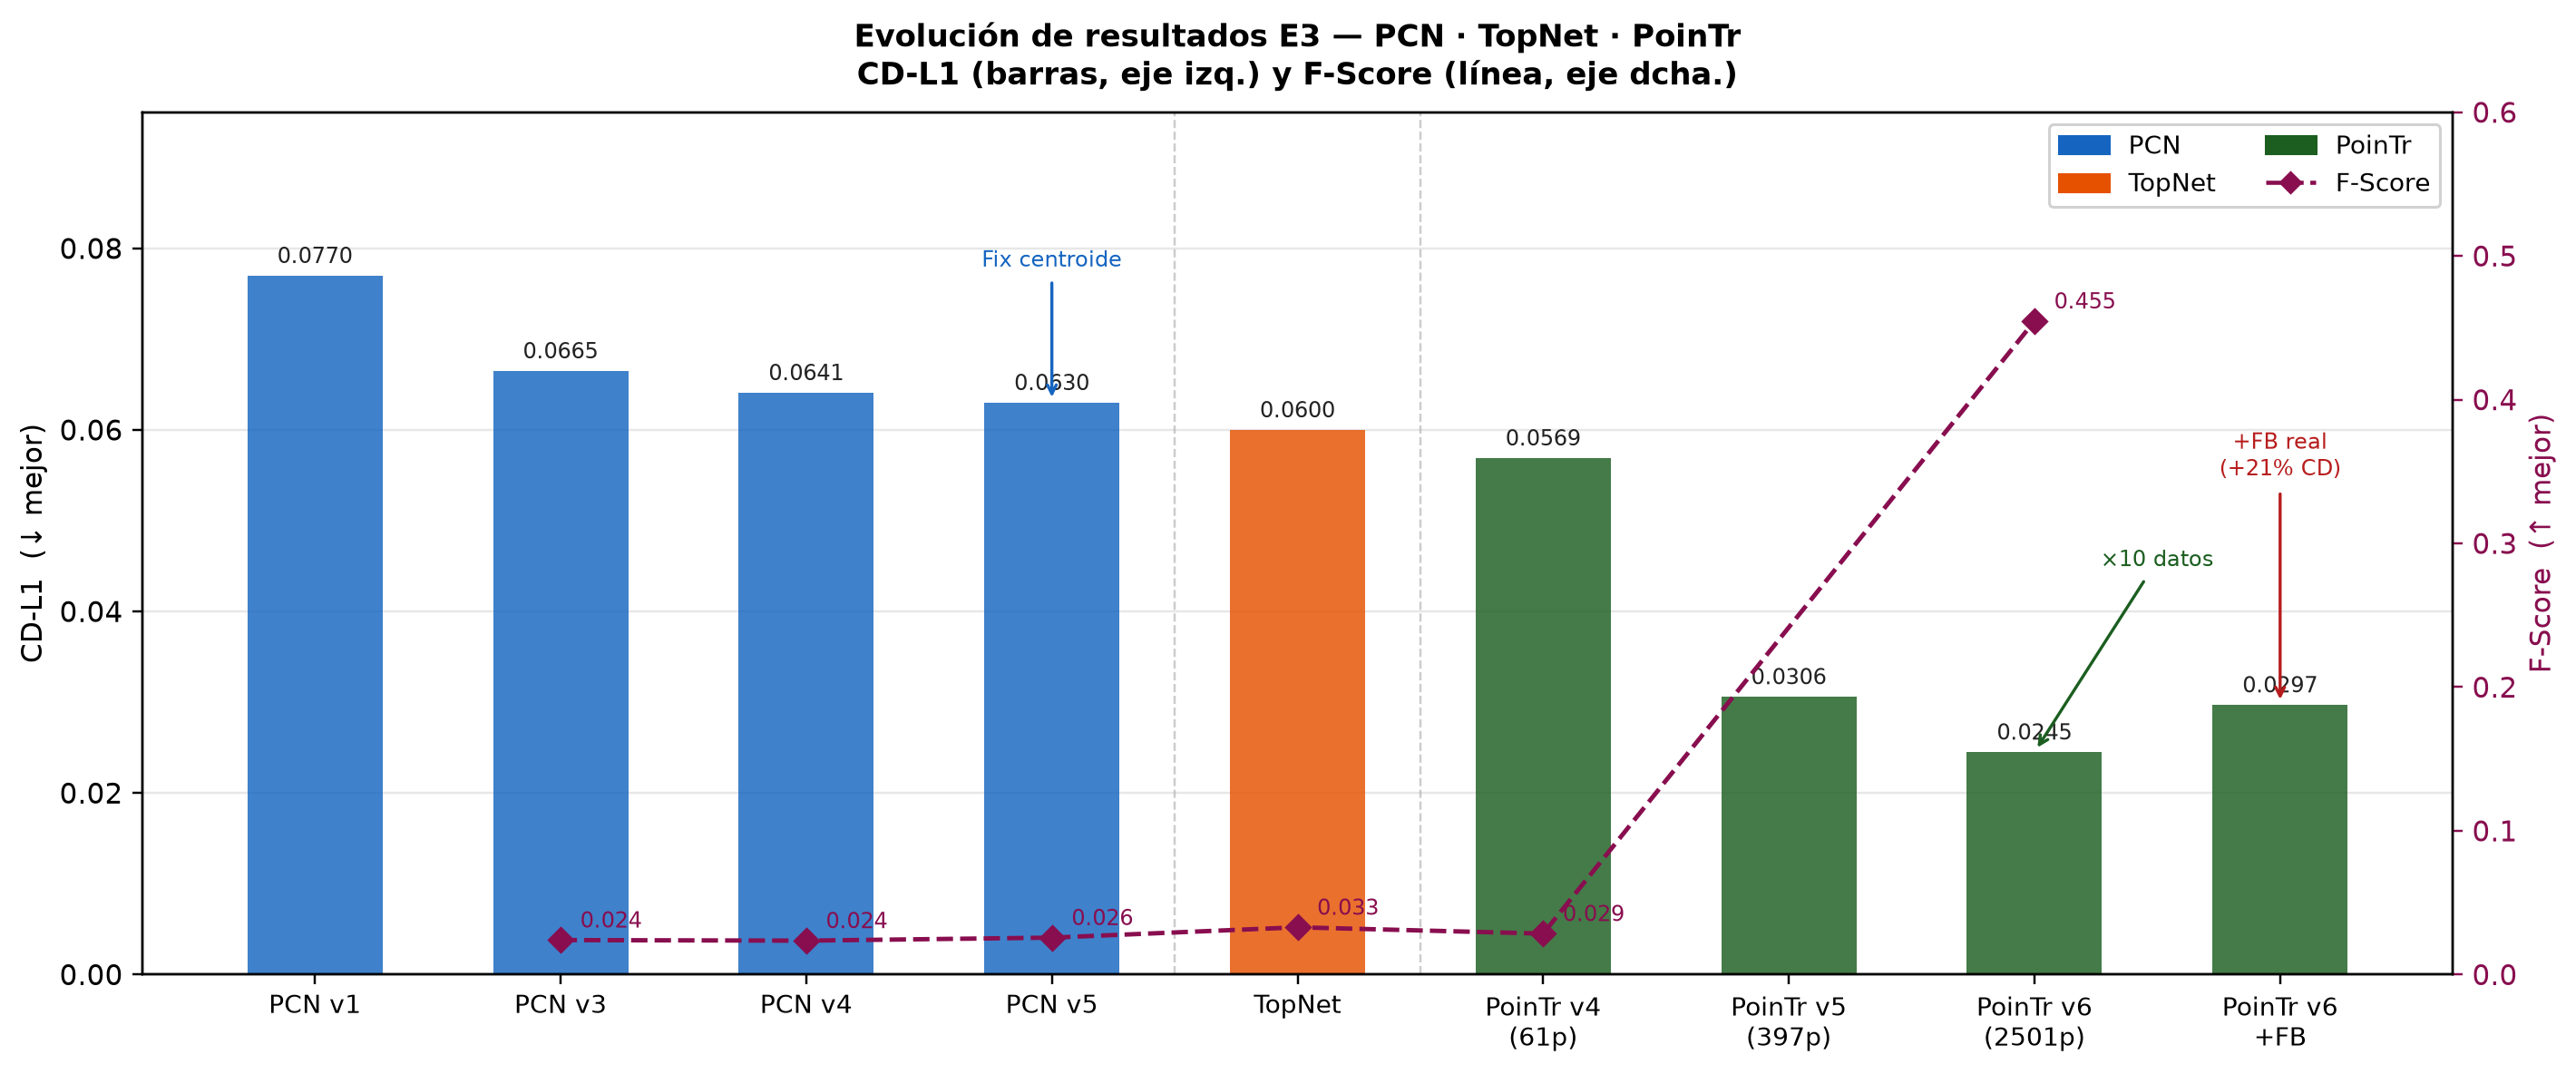
\includegraphics[width=\linewidth]{figura_experimentos_e3}
  \caption{Evolución de CD-L1 ($\downarrow$, barras) y F-Score ($\uparrow$, línea
           discontinua) a lo largo de todos los experimentos de E3.}
  \label{fig:evolucion_e3}
\end{figure}

\subsection{Análisis del mejor modelo (v6\_obj\_sn)}
\label{subsec:mejor_modelo}

El modelo \textbf{v6\_obj\_sn} se entrenó con Objaverse~v2 (397 pares) y ShapeNet
(2.104 pares), durante 500 épocas en una GPU NVIDIA A100-SXM4-40\,GB.
El mejor \textit{checkpoint} se alcanzó en la \textbf{época 486 de 500}, con la pérdida
de validación todavía descendiendo levemente.
Los resultados globales sobre el test set (251 muestras independientes) son
CD-L1~$= \mathbf{0{,}0245}$ y F-Score~$= \mathbf{0{,}4547}$.

El análisis detallado por objeto se recoge en la Tabla~\ref{tab:analisis_objeto}
del Anexo~\ref{ap:tablas}.
Entre el 78\,\% y el 92\,\% de los puntos predichos caen dentro del umbral de corrección
de~0,05 unidades normalizadas.
Los objetos de ShapeNet producen consistentemente mejores resultados que los de Objaverse,
lo que refleja que ShapeNet tiene mallas más uniformes y regularmente muestreadas.

Los 6 mejores objetos del test set por CD-L1 se recogen en la
Tabla~\ref{tab:top6} del Anexo~\ref{ap:tablas}.

\subsubsection*{Visualización de reconstrucciones}

Las figuras~\ref{fig:mejores1}--\ref{fig:peores2} muestran ejemplos representativos
del test set.

\begin{figure}[H]
  \centering
  \begin{tabular}{cc}
    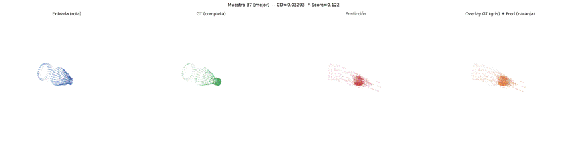
\includegraphics[width=0.45\linewidth]{recon_mejor1} &
    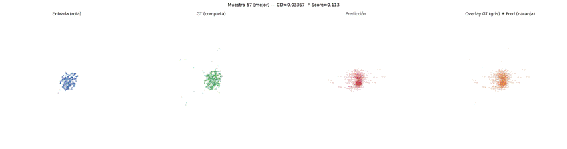
\includegraphics[width=0.45\linewidth]{recon_mejor2} \\
    \small \textbf{Mejor \#1:} CD$=0{,}0329$, F$=0{,}122$ &
    \small \textbf{Mejor \#2:} CD$=0{,}0337$, F$=0{,}113$ \\[6pt]
    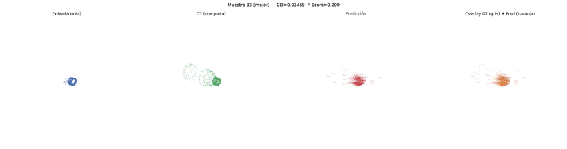
\includegraphics[width=0.45\linewidth]{recon_mejor3} &
    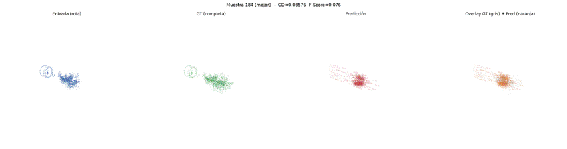
\includegraphics[width=0.45\linewidth]{recon_mejor4} \\
    \small \textbf{Mejor \#3:} CD$=0{,}0346$, F$=0{,}200$ &
    \small \textbf{Mejor \#4:} CD$=0{,}0358$, F$=0{,}076$ \\
  \end{tabular}
  \caption{Los 4 mejores casos del test set por CD-L1 (PoinTr v6\_obj\_sn).}
  \label{fig:mejores1}
\end{figure}

\begin{figure}[H]
  \centering
  \begin{tabular}{cc}
    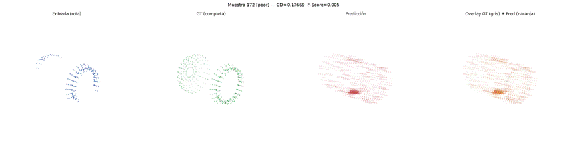
\includegraphics[width=0.45\linewidth]{recon_peor1} &
    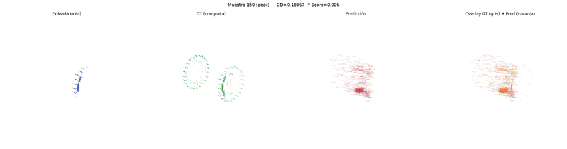
\includegraphics[width=0.45\linewidth]{recon_peor2} \\
    \small \textbf{Peor \#1:} CD$=0{,}177$, F$=0{,}005$ &
    \small \textbf{Peor \#2:} CD$=0{,}181$, F$=0{,}006$ \\[6pt]
    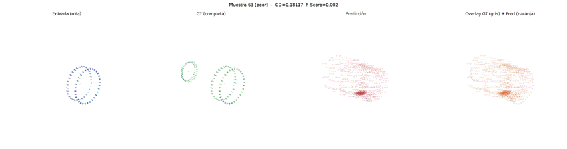
\includegraphics[width=0.45\linewidth]{recon_peor3} &
    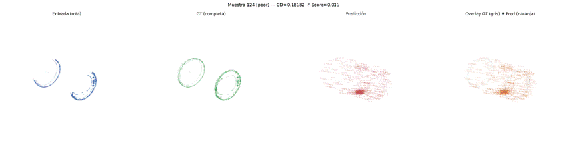
\includegraphics[width=0.45\linewidth]{recon_peor4} \\
    \small \textbf{Peor \#3:} CD$=0{,}181$, F$=0{,}002$ &
    \small \textbf{Peor \#4:} CD$=0{,}182$, F$=0{,}011$ \\
  \end{tabular}
  \caption{Los 4 peores casos del test set por CD-L1 (PoinTr v6\_obj\_sn).}
  \label{fig:peores2}
\end{figure}

% ── 6.7 ─────────────────────────────────────────────────────────────────────
\section{Comparativa global de arquitecturas}
\label{sec:comparativa}

\begin{table}[H]
  \centering
  \caption{Comparativa final entre las tres arquitecturas evaluadas en E3.}
  \label{tab:comparativa_arq}
  \begin{tabular}{lcccccc}
    \toprule
    Modelo & Params. & Encoder & Decoder & CD-L1 $\downarrow$ & F-Score $\uparrow$ & Mejor ép. \\
    \midrule
    PCN v5 (Raquel)         & $\sim$4\,M  & PointNet MLP & FoldingNet 2D   & 0,0630 & 0,026  & 445/500 \\
    TopNet v1 (Rocío)$^*$   & $\sim$5\,M  & PointNet MLP & Árbol jerárquico & 0,0795 & ---   & 359     \\
    \textbf{PoinTr v6\_obj\_sn} & \textbf{42\,M} & \textbf{DGCNN+Transf.} &
      \textbf{Transf.+Fold.} & \textbf{0,0245} & \textbf{0,4547} & \textbf{486/500} \\
    \bottomrule
  \end{tabular}
  \begin{tablenotes}\footnotesize
    \item $^*$ TopNet reportado como \textit{val\_loss} (no CD test independiente).
          PoinTr v6\_obj\_sn: CD test sobre 251 muestras independientes.
  \end{tablenotes}
\end{table}

\textbf{PCN $\to$ TopNet: el \textit{decoder} como cuello de botella.}
Sustituir solo el \textit{decoder} de PCN por un árbol jerárquico produce mejora moderada
(CD 0,063$\to$0,060; F-Score 0,026$\to$0,033).
Confirma que el \textit{decoder folding} de PCN limitaba el rendimiento, pero el vector
global de 1.024\,dim de PointNet tampoco basta para la geometría local requerida.

\textbf{TopNet $\to$ PoinTr: el \textit{encoder} como cuello de botella más importante.}
El salto cualitativo llega al sustituir también el \textit{encoder} por atención
(DGCNN + Transformer): PoinTr reduce el CD un 69\,\% respecto a TopNet y multiplica
el F-Score $\times14$.
Confirma que, para \textit{shape completion}, la arquitectura \textit{transformer} supera
claramente a los enfoques basados en PointNet.

\textbf{Modelo final: PoinTr v6\_obj\_sn}, entregado a E4 y usado en producción con
nubes reales de E2.

% ============================================================
\chapter{Generación de malla imprimible}
\label{ch:malla}

\section{Integración con E3: formato de entrada a E4}
\label{sec:formato_e4}

La etapa E4 recibe como entrada la nube de puntos completa producida por PoinTr.
El formato difiere ligeramente de los 2.048 puntos del contrato E2$\to$E3:
\begin{itemize}
  \item PoinTr genera internamente una nube de predicción de 2.048 puntos que representa
        la región faltante.
  \item La salida final del modelo es la \textbf{concatenación} de la nube parcial de
        entrada con esa predicción.
        El resultado tiene entre 3.700 y 3.900 puntos tras el filtrado de
        \textit{outliers} aplicado ($K=20$, \textit{ratio}$=1{,}5$).
\end{itemize}

Esta mayor densidad respecto al contrato E2$\to$E3 mejora la cobertura de la superficie
en E4, aunque el problema de densidad insuficiente sigue siendo el factor limitante.

% ── 7.2 ─────────────────────────────────────────────────────────────────────
\section{Pipeline de conversión: nube de puntos a STL}
\label{sec:pipeline_stl}

La salida de PoinTr no es directamente imprimible: una impresora 3D necesita una malla
poligonal cerrada.
E4 convierte la nube en STL mediante:

\begin{center}
  nube $\to$ \textbf{Reconstrucción Poisson} $\to$
  \textbf{Reparación topológica} $\to$
  \textbf{Escalar a mm} $\to$ STL + \texttt{report.json}
\end{center}

\textbf{Reconstrucción de superficie (Poisson~\citep{kazhdan2013screened}).}
Se transforma la nube dispersa en malla continua con \textit{Screened Poisson Surface
Reconstruction} (pymeshlab, \texttt{depth}$=10$).
Se generan mallas de 20.000--48.000 vértices y 40.000--96.000 triángulos.

\textbf{Escalar a milímetros.}
El modelo trabaja en unidades normalizadas (esfera radio~1).
Antes de exportar, cada malla se centra y se escala para que su dimensión mayor sea
100\,mm.

% ── 7.3 ─────────────────────────────────────────────────────────────────────
\section{Reparación topológica (manifold3d + pymeshlab)}
\label{sec:reparacion}

La malla de Poisson rara vez cumple los requisitos de impresión sin reparación.
Defectos habituales: aristas no-manifold, huecos, normales inconsistentes y componentes
desconectados, típicamente en zonas de baja densidad de puntos.
Pipeline de reparación en cascada:
\begin{enumerate}
  \item \textbf{Componente principal:} se conserva solo el fragmento con más caras.
  \item \textbf{ManifoldPlus~\citep{huang2020manifoldplus}:} primer intento de
        reconstrucción topológicamente correcta.
  \item \textbf{Fallback con pymeshlab:} si falla ManifoldPlus, se eliminan caras
        duplicadas/degeneradas, se reparan aristas/vértices no-manifold y se cierran
        huecos en tres pasadas crecientes (hasta 30, 150 y 500 aristas).
  \item \textbf{Relleno residual (trimesh):} cierre final de huecos pequeños.
  \item \textbf{Corrección de normales:} verificación y corrección de la orientación de
        triángulos hacia el exterior.
\end{enumerate}

% ── 7.4 ─────────────────────────────────────────────────────────────────────
\section{Validación para impresión 3D}
\label{sec:validacion}

Cada malla reparada se somete a una validación automática cuyos resultados se guardan
en un archivo \texttt{report.json} junto al STL.

\begin{table}[H]
  \centering
  \caption{Criterios de validación automática de la malla para impresión 3D.}
  \label{tab:validacion}
  \begin{tabularx}{\linewidth}{llX}
    \toprule
    Criterio & Tipo & Descripción \\
    \midrule
    \textit{Watertight} (estanca) & \textbf{Obligatorio} &
      La malla no tiene ningún hueco: toda arista está compartida por exactamente
      dos triángulos. \\
    Volumen positivo & \textbf{Obligatorio} &
      La malla encierra un volumen real con las normales apuntando hacia fuera. \\
    Mínimo de caras ($\geq 100$) & \textbf{Obligatorio} &
      Descarta mallas degeneradas que hubieran colapsado durante la reparación. \\
    Número de Euler $= 2$ & \textit{Informativo} &
      Indica topología de esfera simple (genus~0).
      Un objeto con asa tiene Euler~$= 0$ (genus~1) y también es imprimible. \\
    \bottomrule
  \end{tabularx}
\end{table}

% ── 7.5 ─────────────────────────────────────────────────────────────────────
\section{Resultados y limitaciones}
\label{sec:resultados_e4}

Se procesaron muestras del conjunto de test del modelo v6\_obj\_sn en dos ejecuciones.

\textbf{Primera ejecución (solo ManifoldPlus).}
De 16 mallas procesadas, ManifoldPlus devolvió una malla vacía en 14 casos.
Resultado: 0 de 16 mallas aptas para imprimir.

\textbf{Segunda ejecución (ManifoldPlus + pymeshlab en cascada).}
Al añadir pymeshlab como \textit{fallback}, se procesaron 4 mallas.
Los resultados completos figuran en la Tabla~\ref{tab:resultados_e4} del
Anexo~\ref{ap:tablas}.

El experimento de control con nubes de \textit{ground truth} perfectas se recoge en la
Tabla~\ref{tab:control_gt} del Anexo~\ref{ap:tablas}.

\textbf{Diagnóstico confirmado: la causa es la densidad, no PoinTr.}
Incluso con nubes GT perfectas de 2.048 puntos (sin error de predicción), el pipeline E4
no genera mallas \textit{watertight}.
La causa raíz es estructural: con 2.048 puntos sobre una vasija de radio unitario, el
espaciado medio entre vecinos es $\approx0{,}056$ unidades, dejando huecos que Poisson
rellena inventando geometría interna.

\textbf{Resultado operativo.}
E4 produce mallas de 6.000--32.000 caras con forma reconocible.
Ninguna pasa la validación \textit{watertight} estricta, pero son procesables por
laminadores modernos (Cura, PrusaSlicer) con reparación automática.
El único caso con Euler~$=0$ tiene topología de toro ---correcta para una taza con asa---,
confirmando reconstrucción geométricamente correcta aunque no \textit{watertight}.

\textbf{Limitación de resolución.}
Con 2.048 puntos, zonas como asas, bordes finos y concavidades profundas carecen de
densidad suficiente para que Poisson reconstruya correctamente.
Aumentar la resolución de PoinTr a 4.096+ puntos reduciría este problema directamente.

% ============================================================
\chapter{Conclusiones}
\label{ch:conclusiones}

\section{Limitaciones}
\label{sec:limitaciones}

El \textit{fine-tuning} sobre geometrías rotas mejora de forma notable la capacidad del
modelo (IoU medio de~0,055 a~0,311), pero el resultado sigue siendo parcial: un Dice
de~0,45 indica que la reconstrucción capta la forma general de la fractura sin ajustarse
con precisión a sus bordes, y la dispersión entre objetos es alta ---25 de las 26 tazas
de test mejoran, pero la magnitud de la mejora varía de $+0{,}03$ a $+0{,}62$ de IoU---,
lo que sugiere que el modelo generaliza de forma desigual según la severidad y orientación
del corte.

Dos factores del propio diseño experimental limitan hasta dónde puede llegar esta
adaptación.
Primero, las roturas de entrenamiento y validación (532 variantes) se generaron
sintéticamente mediante cortes planos aleatorios sobre las mismas 172 mallas de partida:
el modelo aprende a reconstruir muchas variantes de fractura, pero siempre sobre la misma
base geométrica limitada.
Segundo, un corte por plano produce un borde de fractura recto y regular, muy distinto de
la geometría irregular y multiaxial de una rotura física real, por lo que no está
garantizado que el rendimiento observado se mantenga sobre fracturas reales.

\section{Trabajo futuro}
\label{sec:trabajo_futuro}

\begin{itemize}
  \item Aumentar la resolución de salida de PoinTr a 4.096 o más puntos para mejorar la
        densidad de la nube entregada a E4 y con ello la calidad de la malla final.
  \item Incorporar datos de Fantastic Breaks de forma ponderada o mediante técnicas de
        \textit{domain adaptation} para mejorar el rendimiento con nubes reales de E2.
  \item Ampliar el conjunto de categorías más allá de vasijas para evaluar la
        generalización del pipeline a otros tipos de objetos.
  \item Explorar variantes de reconstrucción de superficie (por ejemplo, \textit{Neural
        Implicit Functions} o métodos basados en campos de distancia signada) que no
        dependan de la densidad de la nube de entrada.
\end{itemize}

% ============================================================
% ── ANEXO ────────────────────────────────────────────────────────────────────
% ============================================================
\appendix
\chapter{Tablas de resultados}
\label{ap:tablas}

Las tablas de este anexo recogen los resultados numéricos completos de las etapas E3
y~E4, cuyo tamaño impediría una lectura cómoda en el cuerpo principal del documento.

% ── A.1 ──────────────────────────────────────────────────────────────────────
\begin{table}[H]
  \centering
  \caption{Todos los experimentos de E3, ordenados por CD-L1 (Tabla~A.1).}
  \label{tab:experimentos_e3}
  \begin{threeparttable}
    \resizebox{\textwidth}{!}{%
    \begin{tabular}{llllrrrcc p{4.5cm}}
      \toprule
      Versión & Modelo & Datos & Limpios & Pares & $N_{\text{test}}$ &
      Mejor ép. & CD-L1 $\downarrow$ & F-Score $\uparrow$ & Observaciones \\
      \midrule
      PCN v1             & PCN    & FB\_v1+sint\_v1       & \xmark & 2.428 & 237 & 97  & 0,0766 & 0,019 & FB v1 desalineado; primer baseline \\
      PCN v3             & PCN    & FB\_v1+sint\_v1       & \xmark & 2.428 & 237 & 347 & 0,0665 & 0,024 & 400 épocas; A100 \\
      PCN v4 (Rocío)$^a$ & PCN    & FB\_v1+sint\_v1       & \xmark & ---   & --- & 150 & 0,0696 &  ---  & val\_loss; mejor PCN Rocío \\
      TopNet v1 (Rocío)$^a$ & TopNet & FB\_v1+sint\_v1    & \xmark & ---   & --- & 359 & 0,0795 &  ---  & val\_loss; mejor TopNet Rocío \\
      PCN v4             & PCN    & FB\_v1+sint\_v2       & \xmark & 2.360 & 236 & 480 & 0,0641 & 0,024 & sint v2: plano+chip+cuña \\
      PCN v5             & PCN    & FB\_v1+sint\_v2       & \ding{115} & 2.360 & 236 & 445 & 0,0630 & 0,026 & CENTRAR=True; mejor PCN Raquel \\
      PoinTr v2          & PoinTr & FB\_v1+sint.filt.     & \xmark & 402   & 41  & 150 & 0,0533 & 0,328$^b$ & F-Score inflado \\
      PoinTr v4          & PoinTr & FB\_v2                & \cmark & 61    & 7   & 285 & 0,0569 & 0,029 & primer exp.\ datos limpios \\
      PoinTr v5\_fb\_obj & PoinTr & FB\_v2+Ob\_v2         & \cmark & 458   & 47  &  ---& 0,0323 & 0,255 & primera combinación real+sint.\ limpio \\
      PoinTr v5\_obj     & PoinTr & Ob\_v2                & \cmark & 397   & 41  &  ---& 0,0306 & 0,270 & sin FB; referencia antes de ShapeNet \\
      PoinTr v6\_fb\_obj\_sn & PoinTr & FB+Ob+SN          & \cmark & 2.562 & 132 &  ---& 0,0297 & 0,387 & añadir FB empeora CD vs.\ v6\_obj\_sn \\
      \rowcolor{rowgray}
      \textbf{PoinTr v6\_obj\_sn} & \textbf{PoinTr} & \textbf{Ob\_v2+ShapeNet} &
        \cmark & \textbf{2.501} & \textbf{251} & \textbf{486/500} &
        \textbf{0,0245} & \textbf{0,4547} & \textbf{MEJOR MODELO; GPU A100 40\,GB} \\
      \bottomrule
    \end{tabular}}
    \begin{tablenotes}\footnotesize
      \item $^a$ Resultados de Rocío reportados como \textit{val\_loss} de entrenamiento
            (no CD test independiente).
      \item $^b$ PoinTr~v2: F-Score inflado por \texttt{CENTRAR\_EN\_ROTO=True} ---
            no comparable con el resto.
      \item Fuente: \texttt{E3/comparar\_experimentos\_EJEC.ipynb} +
            \texttt{E3/colab\_entrenar\_pointr\_v6\_EJEC.ipynb}.
    \end{tablenotes}
  \end{threeparttable}
\end{table}

% ── A.2 ──────────────────────────────────────────────────────────────────────
\begin{table}[H]
  \centering
  \caption{Análisis por objeto del mejor modelo v6\_obj\_sn: puntos correctos vs.\
           erróneos con umbral~$t=0{,}05$ (Tabla~A.2).}
  \label{tab:analisis_objeto}
  \begin{threeparttable}
    \begin{tabular}{lcccc}
      \toprule
      Objeto & CD-L1 & \% correctos ($<0{,}05$) & Puntos erróneos & GT sin cubrir \\
      \midrule
      shapenet\_14588e37\dots & 0,0177 & \textbf{92\,\%} & 311 & 344 \\
      shapenet\_fa23aa60\dots & 0,0233 & 90\,\% & 404 & 202 \\
      shapenet\_f1e43930\dots & 0,0252 & 86\,\% & 554 & 373 \\
      shapenet\_62d897a9\dots & 0,0302 & 86\,\% & 588 & 583 \\
      objaverse\_1095a05d\dots (r0) & 0,0306 & 83\,\% & 700 & 316 \\
      shapenet\_93c83723\dots & 0,0297 & 78\,\% & 896 & 375 \\
      \bottomrule
    \end{tabular}
    \begin{tablenotes}\footnotesize
      \item Umbral: punto correcto = distancia al GT más cercano $< 0{,}05$ unidades
            normalizadas.
      \item Fuente: \texttt{E3/colab\_entrenar\_pointr\_v6\_EJEC.ipynb},
            celda \texttt{cell-viz-error}.
    \end{tablenotes}
  \end{threeparttable}
\end{table}

% ── A.3 ──────────────────────────────────────────────────────────────────────
\begin{table}[H]
  \centering
  \caption{Top~6 objetos del test set por CD-L1 (pipeline\_demo\_EJEC5) (Tabla~A.3).}
  \label{tab:top6}
  \begin{threeparttable}
    \begin{tabular}{clccc}
      \toprule
      N.º & Objeto & CD-L1 $\downarrow$ & F-Score $\uparrow$ & \textit{Outliers} eliminados \\
      \midrule
      \textbf{1} & \textbf{shapenet\_c7fa54dc\dots}    & \textbf{0,0118} & \textbf{0,6249} & \textbf{166} \\
      2          & shapenet\_98d34080\dots               & 0,0124 & 0,5971 & 139 \\
      3          & objaverse\_9770e5a0\dots (r0)         & 0,0127 & 0,6259 & 241 \\
      4          & shapenet\_ee74f5bf\dots               & 0,0134 & 0,5623 & 112 \\
      5          & shapenet\_2927d6c8\dots               & 0,0155 & 0,7436 & 299 \\
      6          & shapenet\_3dbd6642\dots               & 0,0162 & 0,5577 & 338 \\
      \bottomrule
    \end{tabular}
    \begin{tablenotes}\footnotesize
      \item CD medio test set completo (126 pares): 0,0408.
            Peor objeto: CD$=0{,}1878$.
            Nota: este test set usa la partición de la sesión de
            \texttt{pipeline\_demo} (GPU L4 en lugar de A100).
      \item Fuente: \texttt{E4/pipeline\_demo\_EJEC5.ipynb},
            celda \texttt{cell-rankear}.
    \end{tablenotes}
  \end{threeparttable}
\end{table}

% ── A.4 ──────────────────────────────────────────────────────────────────────
\begin{table}[H]
  \centering
  \caption{Resultados E4: 6 objetos seleccionados de la galería (pipeline\_demo\_EJEC5)
           (Tabla~A.4).
           Pipeline: filtrado \textit{outliers} ($K=20$, ratio$=1{,}5$) + suavizado
           Laplaciano ($k=15$, 3 iter) + BPA + Poisson \texttt{depth}$=7$ +
           manifold3d + pymeshlab.}
  \label{tab:resultados_e4}
  \begin{threeparttable}
    \begin{tabular}{clcclrcc}
      \toprule
      N.º & Objeto & CD-L1 & F-Score & Método E4 & Caras & WTight & Euler \\
      \midrule
      1 & shapenet\_f76b14ff\dots   & 0,0184 & 0,4849 & Poisson d7+suav. & 32.503 & \xmark & $-73$ \\
      2 & objaverse\_ca4f9a92\dots  & 0,0208 & 0,5876 & Poisson d7+suav. & 23.483 & \xmark & $-33$ \\
      3 & shapenet\_1ae1ba5d\dots   & 0,0217 & 0,3932 & Poisson d7+suav. & 27.713 & \xmark & $-18$ \\
      4 & shapenet\_24f615dd\dots   & 0,0218 & 0,4993 & Poisson d7+suav. & 26.402 & \xmark & $-47$ \\
      5 & objaverse\_d40aa57b\dots  & 0,0227 & 0,4557 & Poisson d7+suav. & 20.659 & \xmark & $0$ \\
      6 & objaverse\_57be7663\dots (r1) & 0,0232 & 0,2755 & Poisson d7+suav. & 21.666 & \xmark & $-12$ \\
      \bottomrule
    \end{tabular}
    \begin{tablenotes}\footnotesize
      \item 0/6 \textit{watertight}.
            BPA falló en los 6 casos $\to$ todos procesados con Poisson depth$=7$.
            CD medio top-6: 0,0214. CD medio test set completo (126 pares): 0,0408.
      \item Fuente: \texttt{E4/pipeline\_demo\_EJEC5.ipynb},
            celdas \texttt{cell-stl} y \texttt{cell-tabla}.
    \end{tablenotes}
  \end{threeparttable}
\end{table}

% ── A.5 ──────────────────────────────────────────────────────────────────────
\begin{table}[H]
  \centering
  \caption{Experimento de control: mismo pipeline E4 con nubes de \textit{ground truth}
           perfectas (Tabla~A.5).}
  \label{tab:control_gt}
  \begin{threeparttable}
    \begin{tabular}{lrcrrl}
      \toprule
      Objeto & Puntos & Caras & WTight & Euler & Observación \\
      \midrule
      shapenet\_c7fa54dc\dots (GT) & 2.048 & 12.376 & \xmark & $0$    & Topología correcta (toro), no cerrada \\
      shapenet\_98d34080\dots (GT) & 2.048 & 24.293 & \xmark & $-42$  & Geometría interna fantasma \\
      objaverse\_9770e5a0\dots (GT)& 2.048 & 28.491 & \xmark & $-113$ & Euler muy negativo --- mucha geom.\ interna \\
      shapenet\_ee74f5bf\dots (GT) & 2.048 &  8.716 & \xmark & $-23$  & Componente mayor de 3 componentes \\
      shapenet\_2927d6c8\dots (GT) & 2.048 &  6.395 & \xmark & $1$    & Geometría simple --- casi esfera \\
      shapenet\_3dbd6642\dots (GT) & 2.048 & 19.207 & \xmark & $-24$  & Geometría interna fantasma \\
      \bottomrule
    \end{tabular}
    \begin{tablenotes}\footnotesize
      \item 0/6 \textit{watertight} incluso con nubes de GT perfectas.
      \item Fuente: \texttt{E4/pipeline\_demo\_EJEC5.ipynb},
            celda \texttt{cell-diag}.
    \end{tablenotes}
  \end{threeparttable}
\end{table}

% ============================================================
% ── Bibliografía ─────────────────────────────────────────────────────────────
% ============================================================
\bibliographystyle{apalike}
\bibliography{referencias}

\end{document}



